\documentclass{bmstu}

\bibliography{biblio}
\begin{document}
	\def\labelitemi{---}
	
	
	\makethesistitle
	{Информатика и системы управления}
	{Программное обеспечение ЭВМ и информационные технологии}
	{Комбинированный алгоритм продвижения модельного времени при моделировании системы массового обслуживания}
	{ИУ7-86Б}
	{М.~Ф.~Слепокурова} % ФИО студента
	{И.~В.~Рудаков} % ФИО научного руководителя
	{}
	{}
	{Д.~Ю.~Мальцева} % ФИО нормоконтролера
	
	\setcounter{page}{5}
	\begin{essay}{}
Целью данной работы является разработка комбинированного алгоритма продвижения модельного времени и программного обеспечения, реализующего интерфейс для взаимодействия с разработанным алгоритмом.\newline

Для достижения поставленной цели необходимо:
\begin{itemize}
	\item провести анализ предметной области;
	\item проанализировать существующие алгоритмы продвижения модельного времени и обозначить проблему;
	\item разработать комбинированный алгоритм продвижения модельного времени;
	\item реализовать программное обеспечение, реализующее интерфейс для взаимодействия с разработанным алгоритмом;
	\item исследовать разработанный алгоритм и сравнить его с рассмотренными алгоритмами продвижения модельного времени.
\end{itemize}

Результатом выполнения работы является разработанный комбинированный алгоритм продвижения модельного времени, а также реализованное программное обеспечение, предоставляющее интерфейс для взаимодействия с разработанным алгоритмом. Проведенное исследование выявило преимущества и недостатки разработанного алгоритма в сравнении с существующими алгоритмами продвижения модельного времени.
\end{essay}

	
	\maketableofcontents
	
	\chapter*{ВВЕДЕНИЕ}
\addcontentsline{toc}{chapter}{ВВЕДЕНИЕ}

Имитационное моделирование --- это универсальный способ цифрового
представления реальной системы при помощи средств компьютерной техники, вычислительных алгоритмов и технологий программирования. Потребность в имитационном моделировании возникает в связи с дорогими и/или невозможными исследованиями реальных систем. 

На сегодняшний день выделяют три вида имитационного моделирования: агентное моделирование, дискретно-событийное моделирование и системную динамику.
Наиболее развитым подходом среди перечисленных является дискретно-событийное моделирование \cite{economic_system}. При таком подходе не учитывается непрерывная природа событий, и рассматриваются только основные изменения состояния моделируемой системы, а именно события, вызывающие эти изменения. 

Дискретно-событийное моделирование применяется во многих областях, где необходимо анализировать и оптимизировать производительность системы. К областям применения можно отнести производственные системы, логистику, финансовую аналитику, бизнес-процессы, транспортные системы и другие. Дискретно-событийное моделирование может помочь оптимизировать использование ресурсов, повысить эффективность производства, определить оптимальные стратегии управления запасами, маршрутизации транспорта, инвестирования и управления рисками, оптимизировать бизнес-процессы, использование дорожных сетей и многое другое.

Таким образом, имитационное, а в частности дискретно-событийное, моделирование --- мощный инструмент для анализа и оптимизации производительности систем, имеющий применение во множестве различных областей.
	\chapter{Аналитический раздел}
В данном разделе будет проведен анализ предметной области с целью выявления особенностей дискретно-событийного моделирования и распределения событий в реальных системах массового обслуживания. Будут проанализированы существующие алгоритмы продвижения модельного времени, а также формализована постановка задачи в виде IDEF0-диаграммы.

\section{Анализ предметной области}
Многие задачи дискретно-событийного моделирования тесно связаны с теорией
массового обслуживания \cite{imitation_modelling_def}. Объектом изучения теории массового обслуживания (ТМО) являются системы массового обслуживания (СМО). В настоящее время разработано множество математических моделей, позволяющих изучать совершенно различные реально протекающие процессы обслуживания в сфере транспорта, в промышленном производстве, образовании, медицине, военном деле, торговле, телефонии, компьютерных сетях и т.д \cite{gpss}. Модель представляет собой абстрактное описание системы, уровень детализации которой зависит от цели моделирования и возможности получения исходных данных с необходимой точностью \cite{mass_service_systems}. Конечная цель развиваемых в ТМО методов состоит в поиске рациональной структуры обслуживающей системы и ее параметров, а также организации обслуживания, обеспечивающей необходимое его качество.

Под системой массового обслуживания понимают системы, производящие обслуживание поступающих в нее запросов на выполнение каких-либо услуг. Каждая СМО состоит из некоторого числа обслуживающих устройств --- каналов (приборов) обслуживания.
На вход СМО поступает один или несколько потоков запросов (заявок), требующих однотипного обслуживания. К основным элементам СМО относят:
\begin{itemize}
	\item входящий поток заявок;
	\item очередь;
	\item каналы обслуживания;
	\item выходящий поток обслуженных заявок.	
\end{itemize}

Для описания системы массового обслуживания необходимо задать вероятностные законы, определяющие последовательность моментов поступления заявок в систему и продолжительность обслуживания, а также принцип, в соответствии с которым поступающие в систему заявки выбираются из очереди на обслуживание (FIFO, LIFO, случайный отбор и т.д.).

Системы массового обслуживания можно классифицировать по следующим признакам:
\begin{enumerate}
	\item По числу фаз обслуживания --- \textit{однофазные} и \textit{многофазные}.
	\item По числу каналов --- \textit{одноканальные} и \textit{многоканальные}. Многоканальные СМО, в свою очередь, могут подразделяться на \textit{полнодоступные}, подразумевающие однородные каналы (с одинаковыми характеристиками), и \textit{неполнодоступные}, соответственно, с различными характеристиками каналов.
	\item По вероятностным характеристикам времени обслуживания --- \textit{со случайным временем обслуживания} и \textit{с фиксированным постоянным временем обслуживания}.
	\item По характеру случайного процесса, происходящего в СМО --- \textit{маркковские} и \textit{немарковские}. Случайный процесс называется марковским, если для каждого момента времени вероятность любого состояния системы в будущем зависит только от ее состояния в настоящем и не зависит от того, когда и каким образом система пришла в это состояние, т.е. не зависит от того, как процесс развивался в прошлом. Для марковской СМО легко описать математическую модель, однако в реальной жизни таких систем не бывает. Немарковские системы требуют применения статистического моделирования с использованием ЭВМ.
	\item По наличию возможности ожидания обслуживания  --- \textit{с отказами} и \textit{с ожиданием}. В системах с отказами заявка, поступившая в момент, когда все каналы заняты, получает отказ и покидает систему. В системах с ожиданием при занятости всех каналов обслуживания заявка становится в очередь и ждет освобождения одного из каналов. СМО с ожиданием, в свою очередь, можно разделиь на системы \textit{с ограниченным} (по длине очереди или по времени ожидания в очереди) и \textit{неограниченным} ожиданием.
	\item По наличию приоритетов обслуживания --- \textit{без приоритетов} и \textit{с приоритетами}.
	\item По наличию ограничений, накладываемых на поток заявок, --- \textit{замкнутые}, подразумевающие ограниченный поток заявок, которые после обслуживания могут возвращаться в СМО, и \textit{открытые}.
\end{enumerate}


Как уже было сказано ранее, системы массового обслуживания оперируют понятием заявки. Такие события, как поступление новой заявки, начало ее обслуживания и т.д. вызывают изменение состояния системы и образуют \textit{поток событий} --- последовательность однородных событий, следующих одно за другим через некоторые интервалы времени. Такой поток обладает свойством дискретности и носит стохастический характер функционирования ввиду того, что момент попадания новой заявки и время ее обслуживания случайны.

%Период от момента поступления заявки в СМО и до начала обслуживания называется \textit{временем ожидания обслуживания}. Время ожидания обслуживания в совокупности с временем обслуживания составляет \textit{время пребывания требования в системе}.


Для имитацию параллельных событий, происходящих в реальной системе, вводят некоторую глобальную переменную, обеспечивающую синхронизацию всех событий в системе, которую называют модельным (или системным) временем. Для того, чтобы вести отсчет модельного времени и обеспечить правильную хронологическую последовательность наступления основных событий в имитационной модели, используется так называемый таймер модельного времени, который представляет собой переменную для хранения текущего значения модельного времени.

В процессе моделирования системы таймер модельного времени должен постоянно корректироваться в соответствии с основными событиями, возникающими в реальной системе, поэтому одной из важнейших задач имитационного моделирования является \textbf{продвижение модельного времени}.

При рассмотрении реальных СМО можно заметить, что распределение событий в них отнюдь не однородно: события группируются вдоль временной оси \cite{system_modelling}. Начало возникновения групп связано с наступлением некоторого события или их множества. Такой момент времени называется \textit{синхронным моментом}, а наступившее в этот момент событие --- \textit{событием синхронизации}. Интервал, следующий за синхронным моментом времени, обладает плотностью событий, значительно выше средней, и называется \textit{пиковым интервалом}. Причиной появления пиковых интервалов является наличие в системе особых событий, возникновение которых порождает другие события. В качестве примера можно привести синхронизирующие сигналы, переключающие множество триггеров в цифровых сетях.

Рассмотрим временную ось, представленную на рисунке \ref{img:delft_example}. Интервалы вида $[t_i, t_i + t_p]$ $(i = 1, 2, ...)$ являются пиковыми, а точки $t_i$ $(i = 1, 2, ...)$ представляют собой синхронные моменты времени.

\begin{figure}[h!btp]
	\centering
	\includegraphics[width=0.9\columnwidth]{inc/img/delft_example.pdf}
	\caption{Квазисинхронное распределение событий}
	\label{img:delft_example}	
\end{figure}

\textit{Квазисинхронным (пиковым) распределением} событий называется распределение, при котором значение $p$ вероятности возникновения события значительно больше в интервалах времени $[t_i, t_i + t_p]$, чем в промежуточных интервалах $[t_i + t_p, t_{i+1}]$ $(i = 1, 2, ...)$, при $t_{i+1} - t_i > t_p$.

В рассматриваемом случае допускается одновременное возникновение нескольких событий. Также не исключается возможность того, $t_{i+1} - t_i < t_p$ при $t_i \neq i \cdot t_1$.


Алгоритмы продвижения модельного времени должны быть адаптированы под моделирование систем, распределение событий в которых является пиковым.

\section{Алгоритмы продвижения модельного времени}

\subsection{Пошаговый алгоритм}
Данный алгоритм подразумевает продвижение модельного времени на фиксированное $\delta t$ единиц. После каждого обновления часов проверяется, произошли ли какие-либо события в течение предыдущего интервала времени $\delta t$. Если на этот интервал запланировано одно или несколько событий, считается, что данные события происходят в конце интервала, после чего состояние системы и счетчики обновляются соответствующим образом. 

Продвижение времени посредством пошагового алгоритма представлено на рисунке \ref{img:delta_t_example}.

\begin{figure}[h!btp]
	\centering
	\includegraphics[width=0.7\columnwidth]{inc/img/delta_t_example.pdf}
	\caption{Пример продвижения времени посредством пошагового алгоритма}
	\label{img:delta_t_example}	
\end{figure}

Изогнутыми стрелками обозначено продвижение часов модельного времени, а $e_i$ $(i = 1, 2, ...)$ --- это реальное время возникновения события $i$ любого типа.

Рассмотрим несколько представленных интервалов:
\begin{itemize}
	\item в интервале $[0, \delta t)$ событие происходит в момент времени $\delta t$;
	\item в интервале $[\delta t, 2\delta t)$ не происходит ни одного события, однако проверка на наличие событий все равно выполняется;
	\item в интервале $[2\delta t, 3\delta t)$ события происходят в моменты времени $e_2$, $e_3$, однако считается, что они произошли в момент времени $3\delta t$.
\end{itemize}

Заметим, что возникает сложность обработки событий, произошедших в один и тот же временной интервал. Данную проблему можно решить уменьшением размера интервала, однако в таком случае возрастает число проверок возникновения событий, что приводит к значительному увеличению времени выполнения программы. 

Ввиду этой особенности продвижение модельного времени с помощью пошагового алгоритма не используется в тех случаях, когда интервалы времени между последовательными событиями слишком отличны по своей продолжительности \cite{imitation_modelling}. 

Таким образом, продвижение времени посредством постоянного шага имеет два недостатка:
\begin{itemize}
	\item сложность обработки событий, рассматриваемых как одновременные, однако в действительности произошедших в разное время;
	\item  значительные затраты вычислительных ресурсов.
\end{itemize}

В основном этот алгоритм используется для моделирования систем, в которых можно допустить, что все события в действительности происходят в один из моментов $n$ времени $\delta t$ $(n = 0, 1, 2, ...)$ для соответственно выбранного $\delta t$ \cite{imitation_modelling}. 

\subsection{Событийный алгоритм}
При использовании данного алгоритма продвижение модельного времени происходит в моменты возникновения событий в системе.
Предварительно определяется время возникновения будущих событий, после чего таймер модельного времени принимает значение, равное времени возникновения ближайшего события, и в этот момент обновляется состояние системы с учетом произошедшего события, а также сведения о времени  возникновения будущих событий. Затем значение таймера модельного времени продвигается ко времени возникновения нового ближайшего события, аналогично обновляется состояние системы и определяется время будущих событий, и т. д.

Процесс продвижения модельного времени от времени возникновения одного события ко времени возникновения другого продолжается до тех пор, пока не будет выполнено какое-либо заранее установленное условие останова. Поскольку в дискретно-событийной имитационной модели все изменения происходят только во время возникновения событий, периоды бездействия системы просто пропускаются, и часы модельного времени переводятся со времени возникновения одного события на время возникновения другого. При таком подходе длительность интервала продвижения модельного времени от одного события к другому может быть различной.

На рисунке \ref{img:delta_z_example} представлен механизм продвижения модельного времени в системе массового обслуживания с одним устройством обслуживания.

\begin{figure}[h!btp]
	\centering
	\includegraphics[width=0.8\columnwidth]{inc/img/delta_z_example.pdf}
	\caption{Пример продвижения времени посредством событийного алгоритма}
	\label{img:delta_z_example}	
\end{figure}

Рассмотрим следующие обозначения:
\begin{itemize}
	\item $t_i$ --- время поступления $i$-й заявки ($t_0 = 0$);
	\item $A_i = t_i - t_{i-1}$ --- время между поступлением заявок $i-1$ и $i$; 
	\item $S_i$ --- время, потраченное устройством на обслуживание требования $i$ (без учета времени задержки заявки в очереди);
	\item $D_i$ --- время задержки $i$-й заявки в очереди;
	\item $c_i = t_i + D_i + S_i$ --- время ухода $i$-й заявки по окончании обслуживания;
	\item $e_i$ --- время возникновения события $i$ любого типа.
\end{itemize}

Допустим, известны законы распределения вероятностей для времени между поступлением заявок $A_i$ и $A_{i+1}$ и для времени обслуживания $S_i$, заданные функциями распределения $F_A$ и $F_S$ соответственно. Тогда значения $A_i$ будут генерироваться на основе $F_A$, а $S_i$ --- на основе $F_S$.
В момент времени $e_0 = 0$ обработчик заявок незанят. После генерации времени поступления первой заявки $A_1$ таймер модельного времени принимает значение времени возникновения следующего (первого) события $e_1 = t_1$. Ввиду того, что в момент поступления в систему первой заявки обработчик заявок незанят, он немедленно начинает обслуживание с задержкой заявки в очереди $D_1 = 0$, изменяя свое состояние на занятое. Время окончания обслуживания заявки $c_1$ вычисляется путем прибавления сгенерированного $S_1$ к $t_1$. 

Время поступления в систему второй заявки $t_2$ определяется по формуле $t_2 = t_1 + A_2$. Если $t_2 < c_1$, как показано на рисунке \ref{img:delta_z_example}, таймер модельного времени принимает значение времени возникновения следующего события $e_2 = t_2$, иначе --- значение окончания обслуживания первой заявки $c_1$. Так как в момент времени поступления новой заявки $t_2$ обработчик заявок находится в состоянии обслуживания предыдущей заявки (занят), число заявок в очереди увеличивается с 0 до 1. В таком случае сохраняется время поступления заявки, однако не генерируется время обслуживания $S_2$. 

Время поступления в систему третьей заявки вычисляется по формуле $t_3 = t_2 + A_3$. Если $с_1 < t_3$, таймер модельного времени принимает значение времени возникновения следующего события $e_3 = c_1$. Когда заявка, обслуживание которой завершено, покидает систему, начинается обслуживание заявки в очереди, при этом длина очереди уменьшается на 1. Время задержки взятой из очереди заявки вычисляется по формуле $D_2 = c_1 - t_2$, а время окончания обслуживания обработчиком --- $c_2 = c_1 + S_2$. Аналогично если $t_3 < c_2$, таймер модельного времени принимает значение времени возникновения следующего события $e_4 = t_3$ и т.д. 

Моделирование может быть завершено, например, по окончании обслуживания заданного числа заявок или по истечении заданного максимального времени моделирования.


Данный алгоритм целесообразно использовать при моделировании систем, в которых события распределены во времени неравномерно или в тех случаях, когда необходимо точное определение или квазипараллельная обработка одновременных событий \cite{imitation_modelling}.

\section{Оценка сложности алгоритмов}
Сложность рассмотренных алгоритмов в общем зависит от вида распределения событий в моделируемой системе, от их количества, а также от общего времени моделирования.
Заметим, что сложность пошагового алгоритма также зависит от количества блоков, генерирующих события в системе, т.к. при каждом тике времени происходит полный обход всех блоков системы для проверки наличия нового события.

\subsection{Пошаговый алгоритм}
Приняв минимальный тик таймера модельного за времени за единицу, будем считать, что пошаговый алгоритм, используя это значение в качестве $\Delta t$, исключает возможность пропуска событий.

Оценка алгоритмической сложности пошагового алгоритма продвижения модельного времени зависит от количества операций, которые необходимо выполнить при каждом тике таймера модельного времени. Для системы с множеством блоков сложность может быть оценена как $O(N*M)$, где $N$ --- общее время моделирования, выраженное в тиках таймера, а $M$ --- количество операций, необходимых для обработки каждого тика (пропорционально количеству блоков, генерирующих события в моделируемой системе).

\subsection{Событийный алгоритм}
Событийный алгоритм представляет собой обход сортированного списка (очереди с приоритетом) с последующим добавлением в этот же список (очередь) новых событий. Приоритет событий в очереди определяется временем возникновения события в системе.
В худшем случае при обработке одного события в очередь будут добавлены два новых события --- событие об окончании генерации новой заявки и событие об окончании обработки заявки. Для оценки сложности алгоритма необходимо учесть сложность операций вставки и получения элемента в очередь с приоритетом.


Алгоритмическая сложность вставки элемента в очередь с приоритетом зависит от реализации очереди. Наиболее распространенная реализация очереди с приоритетом  --- куча (heap) \cite{priority_queue_implementation}. Сложность операции вставки элемента в такую очередь с приоритетом составляет $O(log N)$, где $N$ - количество элементов в очереди \cite{priority_queue_complexity}. При использовании других реализаций (например, на основе бинарного или сбалансированного дерева), сложность операции вставки элемента может быть другой, однако не хуже приведенной выше  \cite{priority_queue_implementation}.


Сложность получения элемента из очереди с приоритетом имеет алгоритмическую сложность $O(1)$, ввиду того, что корень кучи всегда содержит элемент с наивысшим приоритетом \cite{priority_queue_implementation}.
В других реализациях очереди с приоритетом сложность операции получения элемента может быть выше, например, $O(\log{N})$, где $N$ --- количество элементов в очереди \cite{priority_queue_implementation}. Это связано с тем, что при поиске элемента с наивысшим приоритетом может потребоваться пройти по дереву от корня до листа, что занимает логарифмическое время.
В данной работе рассматривается событийный алгоритм, использующий для списка будущих событий очередь с приоритетом, основанную на куче, ввиду чего сложность операций вставки и получения события составляет соответственно $O(\log{N})$ и $O(1)$.


Тогда оценка алгоритмической сложности событийного алгоритма продвижения модельного времени зависит от общего количества обрабатываемых событий и, с учетом рассмотренной выше реализации, может быть оценена как $O(N\log{N})$, где $N$ --- количество событий, обрабатываемых за указанное время моделирования.

\subsection{Выводы}
На основе приведенной оценки сложности алгоритмов можно сделать вывод о том, что временная эффективность алгоритмов стремительно падает в случае пикового распределения событий в моделируемой системе. Падение эффективности тем больше, чем большее количество блоков, генерирующих события, содержит система.
Пошаговый алгоритм становится тем неэффективнее, чем больше длина временных промежутков между пиковыми интервалами, ввиду невозможности пропустить временные промежутки, не содержащие событий. Событийный же алгоритм стремительно теряет эффективность из-за высокой плотности событий на пиковых интервалах, ввиду роста сложности вставки событий в список будущих событий.

\section{Постановка задачи}
Таким образом, необходимо разработать алгоритм, рассчитанный на моделирование сложных систем (состоящих из большого числа блоков), распределение событий в которых является пиковым. Алгоритм, комбинирующий в себе особенности пошагового и событийного алгоритма, должен решить проблемы падения временной эффективности по причинам, приведенным в предыдущем пункте.

IDEF0-диаграмма для комбинированного алгоритма продвижения модельного времени представлена на рисунках \ref{img:IDEF0-A0} \ref{img:IDEF0-A1}.

\begin{figure}[h!btp]
	\centering
	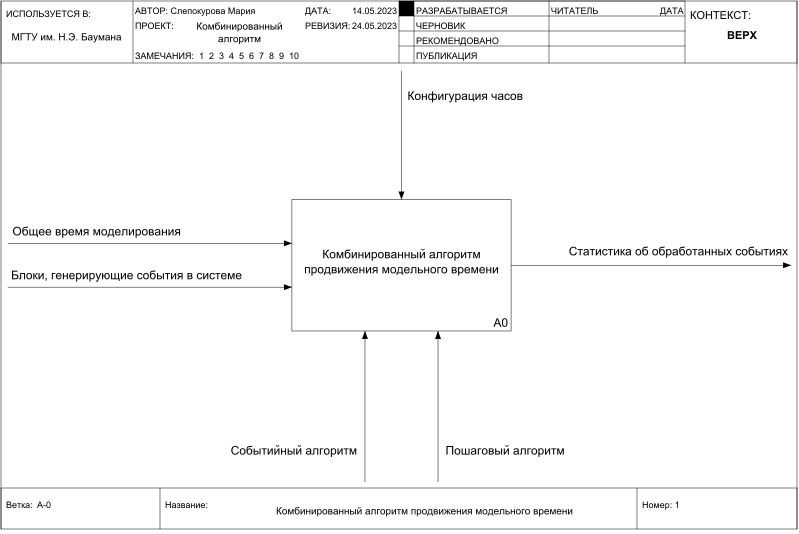
\includegraphics[width=1\columnwidth]{inc/img/IDEF0-A0.png}
	\caption{IDEF0 нулевого уровня}
	\label{img:IDEF0-A0}	
\end{figure}

\begin{figure}[h!btp]
	\centering
	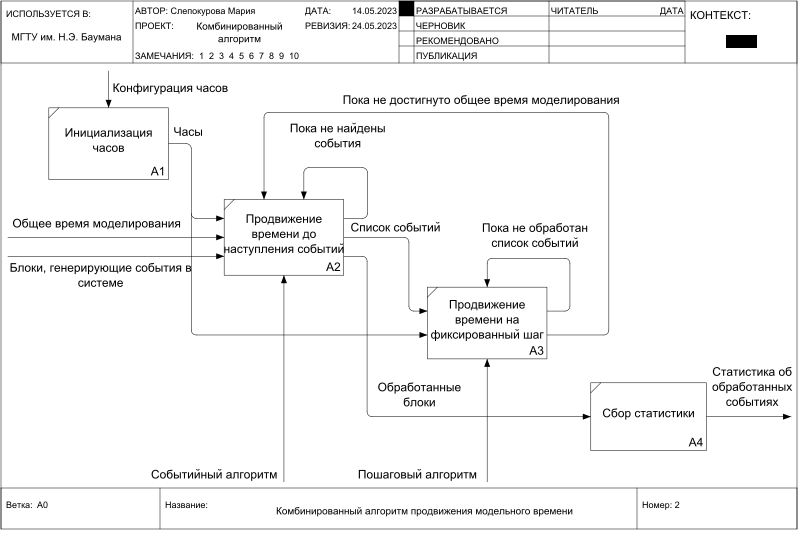
\includegraphics[width=1\columnwidth]{inc/img/IDEF0-A1.png}
	\caption{IDEF0 первого уровня}
	\label{img:IDEF0-A1}	
\end{figure}

\section{Выводы}
В рамках данного раздела были рассмотрены существующие алгоритмы продвижения модельного времени. Была проведена оценка сложности рассмотренных алгоритмов, а также выявлены их недостатки в контексте проанализированной предметной области. На основе полученных заключений была сформулирована цель данной работы, а также формализована постановка задачи в виде IDEF0-диаграммы.

	\chapter{Конструкторский раздел}

\section{Комбинированный алгоритм}
С учетом выявленных недостатков пошагового и событийного алгоритмов предлагается реализовать комбинированный алгоритм таким образом, чтобы на пиковых интервалах он приближался к пошаговому алгоритму, а в промежуточных --- к событийному с большим шагом. Таким образом, проблема неэффективности пошагового алгоритма решается использованием подхода событийного алгоритма на промежуточных интервалах. Однако для решения проблем событийного алгоритма, а именно --- растущей сложности операций вставки и получения событий в список будущих событий, необходимо реализовать структуру для хранения событий более эффективным способом.

\section{Часовая структура данных}
Предлагается реализовать структуру данных для хранения событий, сложность операций вставки и получения элементов для которой будет составлять $O(1)$.

На рисунке \ref{img:hybrid_structure} представлена разработанная для этой задачи структура данных. В основу положена идея об иерархической системе контроля времени, управляемой событиями (HECTAS) \cite{system_modelling_eng}.

\begin{figure}[h!btp]
	\centering
	\includegraphics[width=1\columnwidth]{inc/img/hybrid_structure.pdf}
	\caption{Часовая структура данных для хранения событий}
	\label{img:hybrid_structure}	
\end{figure}

Часовая структура представлена многоуровневой системой списков событий. Каждая ячейка системы --- связный список событий. 

Нулевой уровень представлен массивом таких списков и имеет длину $N_1$. События, попадая на нулевой уровень, обрабатываются аналогично пошаговому алгоритму: временной шаг между соседними ячейками равен минимальному тику таймера модельного времени (единице). Для оптимального моделирования системы с квазисинхронным распределением рекомендуется подобрать длину нулевого уровня таким образом, чтобы она покрывала максимальную длину пиковых интервалов.

Ненулевые уровни системы объединены в массив, каждый уровень, аналогично нулевому, представлен массивом списков событий с фиксированной длиной $N_2$, отличной от длины нулевого уровня (совпадение размерностей допустимо). Для удобства массив уровней будет называться далее таблицей событий. Первая ячейка каждого уровня таблицы описывает временной диапазон от 1 до максимального значения предыдущего уровня. Временной шаг на каждом уровне (гранулярность уровня) совпадает с вместимостью предыдущего уровня.

Гранулярность уровня можно рассчитать по формуле:
\begin{equation}
	G(\text{level}) = 
	\begin{cases}
		1 & \text{, level = 0,} \\
		N_1 N_2^{\text{level}-1} & \text{, иначе,}
	\end{cases}
\end{equation}
где: \\
$N_1$ --- размер нулевого уровня часовой структуры, \\
$N_2$ --- размер табличного уровня часовой структуры. \\ \\


%Обход такой структуры при моделировании системы начинается с верхнего уровня таблицы. В случае обнаружения событий в текущей ячейке таблицы происходит спуск по таблице событий: обнаруженные события размещаются в ячейках предыдущего уровня, после чего происходит аналогичный обход

Необходимое количество уровней в зависимости от требуемого времени моделирования может быть рассчитано по формуле:
\begin{equation}
	k(\text{maxTime}) = \frac{\text{maxTime}} {N_1} \text{,}	\\
\end{equation}
где: \\
maxTime --- общее время моделирования системы. \\ \\

Для вставки события в часовую структуру необходимо рассчитать столбец и уровень нужной ячейки. Нумерация столбцов начинается с 1, как и нумерация уровней в таблице.

Для определения уровня, в который нужно поместить новое событие, необходимо воспользоваться следующей формулой:

\begin{equation}
	\text{Level}(\text{time}) =  \lceil \log_{N_2} \frac{\text{time}}{N_1} \rceil \text{,} \\
\end{equation}
где: \\
time --- время возникновения события. \\ \\

Для определения столбца, в который нужно поместить новое событие, необходимо предварительно определить уровень, после чего воспользоваться следующей формулой:

\begin{equation}
	\text{Column(time, level)} = 
	\begin{cases}
		(\text{time} - 1) \mod N_1 + 1 & \text{, level = 0,} \\
		\lceil \frac{\text{time}}{G(\text{level})} \rceil & \text{, иначе,}
	\end{cases}
	\label{eq:column}
\end{equation}
где: \\
$N_1$ --- размер нулевого уровня часовой структуры, \\
$G(\text{level})$ --- гранулярность уровня level. \\ \\

Подбор значений $N_1$ и $N_2$ зависит от требований, предъявляемых к моделируемой системе. Как уже говорилось ранее, в случае квазисинхронного распределения в системе значение $N_1$ следует подобрать таким образом, чтобы оно покрывало максимальный размер пикового интервала. Для $N_2$ же наиболее оптимальным значением будет 10: ввиду множества операций взятия логарифма по основанию $N_2$ возможно использование оптимизированных реализаций взятия десятичного алгоритма. Очевидно, при увеличении обоих величин масштабирование времени в часовой структуре будет больше, что приведет к уменьшению количества уровней в таблице и, как следствие, к уменьшению операций, связанных с перемещением списков событий с одного уровня на другой.


Для наглядности на рисунке \ref{img:hybrid_structure_example} приведен пример заполненной часовой структуры с размеров нулевого уровня $N_1 = 15$, размером табличного уровня $N_2 = 10$ и количеством уровней таблицы $k = 3$.

\begin{figure}[h!btp]
	\centering
	\includegraphics[width=1\columnwidth]{inc/img/hybrid_structure_example.pdf}
	\caption{Часовая структура данных для хранения событий}
	\label{img:hybrid_structure_example}	
\end{figure}

Видно, насколько сильно масштабируется время на верхних уровнях даже при такой небольшой размерности $N_1$. Если при тех же $k$ и $N_2$ взять $N_1$ равным, например, 100, то максимальное время моделирования, описываемое такой структурой, будет достигать 1 млн тиков таймера модельного времени.

\section{Описание алгоритма}
Прежде всего необходимо инициализировать часовую структуру в соответствии с требованиями, предъявляемыми к моделируемой системе. Оптимальный подбор значений описан в предыдущем пункте.

При дальнейшем описании алгоритма будет называть генератором блок системы, который генерирует заявки, а процессором --- блок, который обрабатывает заявки.


Перед началом процесса моделирования необходимо <<запустить>> все генераторы системы, т.е. начать генерацию заявок и поместить в часовую структуру события, связанные с окончанием генерации этих заявок.
На этом этапе (инициализации) события помещаются в ячейки верхнего уровня таблицы событий, однако все последующие события, сгенерированные блоками моделируемой системы размещаются либо в ячейке нулевого уровня, либо в таблице событий, в зависимости от текущего времени и времени возникновения события.


Процесс моделирования представляет собой рекурсивный обход уровней часовой структуры и начинается с верхнего уровня. Текущая ячейка проверяется на наличие событий: если события не найдены, текущее значение таймера увеличивается на гранулярность текущего уровня, иначе начинается обработка списка событий.

Обработка списка событий заключается в последовательном <<спуске>> всех событий на уровень ниже до тех пор, пока не будет достигнут нулевой уровень. Для каждого события из рассматриваемого списка происходит пересчет столбца для уровня ниже. Для этого необходимо пересчитать время события в рамках уровня, на который происходит перемещение. Сделать это можно, использовав следующую формулу:

\begin{equation}
	\text{time'}(\text{level}) =  \text{time} \mod G(\text{level}) + 1 {,} \\
\end{equation}
где: \\
time --- время возникновения события, \\
$G(\text{level})$ --- гранулярность уровня, с которого происходит спуск события. \\ \\

Тогда пересчет столбца для уровня ниже может быть осуществлен с помощью формулы \ref{eq:column} как $\text{Column}(\text{time'}, \text{level} - 1)$.

После спуска списка событий по уровню, на который были перемещены события, осуществляется такой же проход, как и по верхнему: в случае нахождения не пустой ячейки происходит последовательный спуск на уровень ниже, а иначе --- продвижение времени на гранулярность текущего уровня.

Обработка каждого события происходит непосредственно на нулевом уровне часовой структуры. Перед тем, как начать обход нулевого уровня, необходимо определить его текущее окончание временного диапазона. Сделать это можно по формуле:

\begin{equation}
	\text{currentEnd} = \text{currentTime} + N_1 {,} \\
\end{equation}
где: \\
currentTime --- текущее значение таймера модельного времени, \\
$N_1 $ --- размер нулевого уровня часовой структуры. \\ \\

Гранулярность нулевого уровня всегда равна минимальному значению тика модельного времени, т.е. 1, так что при обходе нулевого уровня значение таймера модельного времени инкрементируется, аналогично пошаговому алгоритму. Каждая ячейка нулевого уровня проверяется на наличие событий:
если событие найдено, происходит его обработка, иначе --- переход к следующей ячейке с увеличением значения таймера.

При обработке каждого события (окончание генерации заявки и окончание обработки заявки) происходит создание и добавление в часовую структуру новых событий: о следующем окончании генерации и о следующем окончании обработки заявки. При добавлении нового события необходимо прежде всего проверить, есть ли возможность поместить его на нулевом уровне, сравнив значение времени возникновения события со значением текущего окончания временного диапазона, описываемого нулевым уровнем ($currentEnd$). В случае, если время нового события не превышает это значение, новое событие помещается на нулевой уровень в столбец $Column(time, 0)$, иначе для нового события предварительно вычисляется номер уровня, после чего уже рассчитывается номер столбца ячейки таблицы. События, размещенные таким образом на нулевом уровне будут обработаны во время текущего <<пошагового>> прохода.

По завершении обхода нулевого уровня происходит рекурсивный возврат на предыдущие по следованию уровни, после чего аналогично продолжается их обход. В итоге произойдет возврат в уже пустую ячейку верхнего уровня.

Может возникнуть ситуация, при которой по возвращении в ячейку таблицы список событий, содержащийся в этой ячейке все еще будет непустым. Это происходит ввиду генерации новых событий во время обработки уже существующих. Для обработки таких кейсов введена переменная, содержащая количество повторных обработок текущего уровня --- $retries$, значение которой при первичной обработке ячейки равно 0. 

При обработке непустой ячейки таблицы происходит проверка значения переменной $retries$: если оно равно 0 --- ячейка обрабатывается в первый раз, т.е. происходит обычная, описанная выше, обработка списка событий, иначе --- ячейка обрабатывается повторно и прежде, чем приступать к обработке списка событий, необходимо уменьшить текущее значение таймера модельного времени на величину гранулярности обрабатываемого уровня. Это необходимо сделать из-за того, что в таком случае произойдет повторный обход пустых ячеек уже обработанных уровней и, соответственно, ложное увеличение модельного времени.

Процесс моделирования завершается по наступлении максимального времени моделирования: при добавлении события в часовую структуру время события сравнивается с максимальным временем, и, в случае превышения лимита, добавление события не происходит. Таким образом, при наступлении максимального времени моделирования произойдет возврат на верхний уровень таблицы событий и обход пустых ячеек, оставшихся на нем.


Результатом работы такого симулятора является собранная со всех блоков системы статистика:
информация о среднем времени генерации/обработки заявки, общее количество сгенерированных/обработанных заявок и среднее время ожидания заявки для каждого процессора.

\clearpage
На рисунке \ref{img:hybrid_simulate_schema} представлена схема комбинированного алгоритма продвижения модельного времени. Для удобства часовая структура в схемах называется часами.
\begin{figure}[h!btp]
	\centering
	\includegraphics[width=1\columnwidth]{inc/img/hybrid_simulate_schema.pdf}
	\caption{Схема комбинированного алгоритма}
	\label{img:hybrid_simulate_schema}	
\end{figure}

\clearpage
На рисунке \ref{img:hybrid_processLevel_schema} представлена схема алгоритма обработки одного уровня часовой структуры.
\begin{figure}[h!btp]
	\centering
	\includegraphics[width=1\columnwidth]{inc/img/hybrid_processLevel_schema.pdf}
	\caption{Схема алгоритма обработки одного уровня часовой структуры}
	\label{img:hybrid_processLevel_schema}	
\end{figure}

\clearpage
На рисунке \ref{img:hybrid_moveEvents_schema} представлена схема алгоритма перемещения событий из ячейки часовой структуры на уровень ниже.
\begin{figure}[h!btp]
	\centering
	\includegraphics[width=0.8\columnwidth]{inc/img/hybrid_moveEvents_schema.pdf}
	\caption{Схема алгоритма перемещения событий из ячейки часовой структуры на уровень ниже}
	\label{img:hybrid_moveEvents_schema}	
\end{figure}

\clearpage
На рисунке \ref{img:hybrid_processEvent_schema} представлена схема алгоритма обработки одного события.
\begin{figure}[h!btp]
	\centering
	\includegraphics[width=0.8\columnwidth]{inc/img/hybrid_processEvent_schema.pdf}
	\caption{Схема алгоритма обработки одного события}
	\label{img:hybrid_processEvent_schema}	
\end{figure}

\clearpage
\section{Пошаговый алгоритм}
Пошаговый алгоритм подробно описан в соответствующем пункте аналитического раздела. 

Схема пошагового алгоритма представлена на рисунке \ref{img:delta_t_schema}.

\begin{figure}[h!btp]
	\centering
	\includegraphics[width=0.8\columnwidth]{inc/img/delta_t_schema.pdf}
	\caption{Схема пошагового алгоритма}
	\label{img:delta_t_schema}	
\end{figure}

Используемые обозначения:
\begin{itemize}
	\item $t_M$ --- текущее значение модельного времени;
	\item $Z(t_M)$ --- состояние системы в текущий момент времени;
	\item $T_M$ --- интервал моделирования.
\end{itemize}

\section{Событийный алгоритм}
Событийный алгоритм подробно описан в соответствующем пункте аналитического раздела. 

Схема событийного алгоритма представлена на рисунке \ref{img:delta_z_schema}.

\begin{figure}[h!btp]
	\centering
	\includegraphics[width=1\columnwidth]{inc/img/delta_z_schema.pdf}
	\caption{Схема событийного алгоритма}
	\label{img:delta_z_schema}	
\end{figure}

Используемые обозначения:
\begin{itemize}
	\item $t_M$ --- текущее значение модельного времени;
	\item $Z(t_M)$ --- состояние системы в текущий момент времени;
	\item $T_M$ --- интервал моделирования;
	\item $t_{соб i}$ --- время возникновения $i$-го события.
\end{itemize}

\section{Моделируемая СМО}
В качестве моделируемой системы предлагается рассмотреть модель МФЦ.

Согласно информации, предоставленной официальным сайтом мэра Москвы \cite{mos_ru}, наименее загруженными днями для МФЦ считаются выходные, а максимальная загрузка приходится на вторник. В будние дни наименьшая загрузка наблюдается с 08.00 до 11.00 и с 14.00 до 20.00. Время работы МФЦ --- с 08.00 до 20.00 без перерывов и выходных. Среднее время ожидания приема в центрах госуслуг составляет 3 минуты, максимальное --- 15 минут.

Согласно статье с сайте Портала Правительства Московской области \cite{mosreg_ru} количество окон обслуживания в одном из подмосковных МФЦ было увеличено до 30.

Тогда моделируемая система будет состоять из:
\begin{enumerate}
	\item Автоматов с талонами (4 шт). Время подбора и получения талона клиентом на каждом автомате составляет $15\pm60$ секунд.
	\item Окон обслуживания (до 40 шт). Время обслуживания одного клиента в окне составляет от $10$  до $30$ минут.
	\item Работников архива (10 чел). После обслуживания клиента в одном из окон, информация о предоставленной услуге вместе с данными о нужных документах заносится в систему одним из работников архива. Длительность этого процесса зависит от оказываемой услуги и количества документов, необходимых для подготовки, ввиду чего время обслуживания обладает большим разбросом и может занимать от $5$ до $20$ минут.
\end{enumerate}

Необходимо смоделировать работу такого МФЦ в течение одной недели.


За минимальный шаг времени принимается 1 секунда. Тогда общее время моделирования для 7 12-часовых рабочих дней эквивалентно 302400 секундам. Пиковые интервалы приходятся на время с 11.00 до 14.00, т.е. их длина составляет 10800 секунд (3 часа), а непиковые интервалы приходятся на оставшиеся 9 часов рабочего дня с общей длительностью в 32400 секунды. Ввиду отсутствия в открытом виде статистической выборки по посещаемости МФЦ среднее время появление нового посетителя будем считать 30 секунд для пикового интервала и 420 секунд (7 минут) для непикового. Появление посетителей подчинено экспоненциальному закону.

На рисунке \ref{img:system_modelling_distr}	 представлено распределение для генератора заявок, созданное на основе предоставленной информации о загруженности МФЦ.

\begin{figure}[h!btp]
	\centering
	\includegraphics[width=1\columnwidth]{inc/img/system_modelling_distr.pdf}
	\caption{Распределение событий поступления заявок в МФЦ}
	\label{img:system_modelling_distr}	
\end{figure}

На рисунке \ref{img:system_modelling} представлена схема МФЦ в терминах СМО.

\begin{figure}[h!btp]
	\centering
	\includegraphics[width=1\columnwidth]{inc/img/system_modelling.pdf}
	\caption{Схема МФЦ в терминах СМО}
	\label{img:system_modelling}	
\end{figure}

	
\section{Выводы}
В рамках данного раздела были описаны основные особенности разрабатываемого комбинированного алгоритма продвижения модельного времени. Были изложены ключевые этапы комбинированного, а также пошагового и событийного алгоритмов в виде схем алгоритмов. Также были описаны требования к моделируемой в рамках данной работы системы массового обслуживания.
	\chapter{Технологический раздел}
В данном разделе будет обоснован выбор средств программной реализации алгоритмов. Будет разработано программное обеспечение, реализующее комбинированный алгоритм продвижения модельного времени, выполнено его тестирование.

\section{Выбор средств программной реализации}
Для реализации комбинированного, а также пошагового и событийного алгоритмов был выбран язык программирования Kotlin и графическая библиотека Swing.

Язык Kotlin был выбран по ряду следующих причин:

\begin{enumerate}
	\item \textbf{Простота и выразительность.} Kotlin предлагает чистый и лаконичный синтаксис, предоставляет множество удобных функций и других инструментов, что значительно упрощает реализацию сложных алгоритмов продвижения модельного времени.
	
	\item \textbf{Высокая производительность.} Kotlin компилируется в байт-код JVM, что позволяет достичь высокой производительности. Это важно для алгоритмов модельного времени, которые требуют обработки больших объемов данных и выполнения вычислительно интенсивных операций.
	
	\item \textbf{Кросс-платформенность.} Код, написанный на Kotlin может работать на различных платформах, включая JVM, Android, JavaScript и Native, что открывает множество возможностей для интеграции реализованных алгоритмов в различные системы.
	
	\item \textbf{Поддержка объектно-ориентированного программирования.} Kotlin предлагает гибкую парадигму программирования, которая позволяет использовать как функциональный, так и объектно-ориентированный стиль программирования. С сущностями поставленной задачи продвижения модельного времени удобнее всего работать как с системой классов.
	
	\item \textbf{Богатая экосистема.} Kotlin имеет широкую и активную экосистему инструментов и библиотек, которые могут быть полезны при реализации алгоритмов. К таким библиотекам относится библиотека Swing, предоставляющая инструменты для создания графического интерфейса.
	
	\item \textbf{Безопасность типов.} Kotlin обеспечивает безопасность типов и проверку на этапе компиляции, что сокращает время отладки и повышает стабильность программного обеспечения.
\end{enumerate}


В свою очередь, библиотека Swing была выбрана в связи со следующими преимуществами:

\begin{enumerate}
	\item \textbf{Кросс-платформенность.} Как и Kotlin, Swing является кросс-платформенной библиотекой, что означает, что приложения, созданные с использованием Swing, могут работать на различных операционных системах. Это обеспечивает широкий охват пользователей и удобство разработки.
	
	\item \textbf{Богатый набор компонентов.} Swing предоставляет обширный набор графических компонентов, что позволяет создавать самые разнообразные интерфейсы в зависимости от требований проекта.

	\item \textbf{Простота использования.} Swing предоставляет интуитивно понятный и простой в использовании API. Kotlin, в свою очередь, предлагает лаконичный и выразительный синтаксис. Сочетание этих двух инструментов делает разработку GUI более удобной и эффективной.
	
	\item \textbf{Хорошая документация и сообщество.} Swing имеет обширную документацию и активное сообщество разработчиков. Это облегчает процесс изучения и получения поддержки, а также предоставляет доступ к множеству ресурсов и примеров кода.
\end{enumerate}


\section{Разработка программного обеспечения}

Полный код разработанного программного обеспечения представлен в приложении.

В рамках данного раздела будут рассмотрены основные классы, необходимые для решения поставленной задачи.


В листинге \ref{lst:DurationGenerator} представлен интерфейс \textbf{DurationGenerator}, который реализуют все классы-генераторы продолжительности, например, класс \textbf{UniformDurationGenerator}, представленный в листинге \ref{lst:UniformDurationGenerator}. Метод $generate$ класса \textbf{UniformDurationGenerator} используется для генерирации продолжительность согласно равномерному распределению на основе значений $min$ и $max$, переданных в конструктор. Интерфейс \textbf{DurationGenerator} используется всеми сущностями, реализующими блоки системы, --- процессорами и генераторами, для генерации времени выполнения той или иной операции.
\listingfileKotlin{time/DurationGenerator.kt}{DurationGenerator}
\listingfileKotlin{time/UniformDurationGenerator.kt}{UniformDurationGenerator}

В листинге \ref{lst:Block} представлен интерфейс \textbf{Block}, который реализуют классы \textbf{Processor} и \textbf{Generator}. Метод $cleanupState$ используется для очищение всю статистику и текущее состояние блока. Метод $currentFinishTime$ --- метод-геттер, используемый для получения времени окончания текущего запущенного процесса. Метод $start$ используется для запуска процесса блока: для генератора --- процесса генерации заявки, для процессора --- процесса обработки заявки.
\listingfileKotlin{simulator/Block.kt}{Block}


В листинге \ref{lst:Event} представлен класс \textbf{Event}, описывающий события в моделируемой системе, где $time$ --- время наступления события, $block$ --- блок системы, сгенерировавший событие.
\listingfileKotlin{simulator/Event.kt}{Event}


В листинге \ref{lst:Request} представлен класс \textbf{Request}, описывающий заявки в моделируемой системе, где $timeIn$ --- время поступления заявки в с систему, $timeOut$ --- время выхода заявки из системы.
\listingfileKotlin{simulator/Request.kt}{Request}


В листинге \ref{lst:Processor} представлен класс \textbf{Processor}, описывающий блок процессора в моделируемой системе. Как уже было сказано выше, он реализует интерфейс \textbf{Block}. Рассмотрим подробнее поля класса:
\begin{itemize}
	\item $durationGenerator$ --- генератор продолжительности обработки заявки;
	\item $receivers$ --- список процессоров-получателей обработанной заявки;
	\item $queue$ --- очередь заявок процессора;
	\item $currentRequest$ --- текущая обрабатываемая заявка;
	\item $currentStartTime$ --- время начала обработки текущей заявки;
	\item $currentFinishTime$ --- время окончания обработки текущей заявки;
	\item $totalRequests$ --- общее количество обработанных заявок;
	\item $totalProcessingTime$ --- общее время работы процессора;
	\item $totalWaitingTime$ --- общее время ожидание заявок в очереди.
\end{itemize}
Помимо этого, класс \textbf{Processor} содержит вложенный класс \textbf{Statistics}, описывающий собираемую по процессору статистику --- общее количество обработанных заявок, среднее время обработки заявки и среднее время ожидания заявки в очереди. Статистика вычисляется с помощью метода $statistics$ на основе полученных за время моделирования значений $totalRequests$, $totalProcessingTime$, $totalWaitingTime$.
\listingfileKotlin{simulator/Processor.kt}{Processor}


В листинге \ref{lst:Generator} представлен класс \textbf{Generator}, описывающий блок генератора в моделируемой системе. Как уже было сказано выше, он реализует интерфейс \textbf{Block}. Рассмотрим подробнее поля класса:
\begin{itemize}
	\item $durationGenerator$ --- генератор продолжительности генерации заявки;
	\item $receivers$ --- список процессоров-получателей сгенерированной заявки;
	\item $currentRequest$ --- текущая генерируемая заявка;
	\item $currentStartTime$ --- время начала генерации текущей заявки;
	\item $currentFinishTime$ --- время окончания генерации текущей заявки;
	\item $totalRequests$ --- общее количество сгенерированных заявок;
	\item $totalGenerationTime$ --- общее время работы генератора.
\end{itemize}
Помимо этого, класс \textbf{Generator} содержит вложенный класс \textbf{Statistics}, описывающий собираемую по генератору статистику --- общее количество обработанных заявок и среднее время генерации заявки. Статистика вычисляется с помощью метода $statistics$ на основе полученных за время моделирования значений $totalRequests$, $totalGenerationTime$.
\listingfileKotlin{simulator/Generator.kt}{Generator}


В листинге \ref{lst:Simulator} представлен интерфейс \textbf{Simulator}, который реализуют классы-симуляторы для пошагового, событийного и комбинированного алгоритмов. В интерфейсе представлен вложенный класс \textbf{Statistics}, описывающий собираемую в процессе моделирования статистику. Класс содержит статистику, собранную со всех процессоров и генераторов, а также общее время выполнения симуляции.
\listingfileKotlin{simulator/Simulator.kt}{Simulator}

Листинги классов-симуляторов \textbf{HybridSimulator}, \textbf{TimeBasedSimulator} и \textbf{EventBasedSimulator} приведены в приложении --- \ref{lst:full:HybridSimulator}, \ref{lst:full:TimeBasedSimulator} и \ref{lst:full:EventBasedSimulator} соответственно --- и реализуют описанные алгоритмы продвижения модельного времени.

\subsection{Пример использования разработанного ПО}


\subsection{Моделирование МФЦ}

\subsection{Выводы}
В рамках данного раздела был обоснован выбор программных средств реализации алгоритма. Было разработано программное обеспечение, реализующее комбинированный алгоритм продвижения модельного времени, и описаны ключевые особенности его реализации. Также был разработан пользовательский интерфейс и продемонстрирован пример работы программного обеспечения.
	\chapter{Исследовательский раздел}
Ключевым недостатком пошагового алгоритма в сравнении с комбинированным является невозможность пропустить интервалы времени, не содержащие никаких событий. Как следствие, пошаговый алгоритм плохо адаптирован под квазисинхронное распределение событий, рассмотренное в аналитическом разделе. Событийный алгоритм, в свою очередь, теряет свою временную эффективность при росте очереди событий, а также при увеличении числа обращений к ней ввиду не константной сложности вставки событий.

Для измерения времени выполнения программного обеспечения используется устройство MacBook Air M1, 8-core GPU, 16 ГБ.

Для повышения точности результатов (ввиду наличия фактора случайности в процессе работы программного обеспечения) для каждого набора данных производится 100 прогонов алгоритмов с получением в итоге среднего значения.

\section{Сравнение алгоритмов}

\textbf{Квазисинхронное распределение событий}

Предлагается сравнить временные затраты пошагового, событийного и комбинированного алгоритмов на системе, состоящей из одного генератора и одного процессора. Продолжительность генерации заявки генерируется согласно равномерному квазисинхронному распределению с длиной пикового интервала в 100 тиков, минимальным и максимальным значением в 1 и 2 тика соответственно. Продолжительность обработки заявки генерируется в соответствии с равномерным распределением с минимальным и максимальным значением в 1 и 2 тика соответственно.
Моделируется работа системы в течение 100000 тиков таймера модельного времени. При этом для квазисинхронного распределения изменяется длина непикового интервала времени (интервала между пиками). Для комбинированного алгоритма размер нулевого уровня выбран в соответствии с длиной пикового интервала (100 тиков), а размер ненулевого уровня выбран равным 10. Шаг таймера модельного времени для пошагового алгоритма составляет 1 тик.

На рисунке \ref{img:graph1} представлен график сравнения временных затрат алгоритмов в зависимости от длины непиковых интервалов.

\begin{figure}[H]
	\centering
	\begin{tikzpicture}
		\begin{axis}[
			width=15cm,
			height=10cm,
			grid=major,
			grid style=dashed,
			axis lines=left,
			ylabel={Время работы, мс},
			xlabel={Длина непикового интервала, тик},
			xmin=0, ymin=0,
			xmax=3000, ymax=500,
			xtick={0,500,...,3000},
			legend pos=north west
			]
			\addplot[color=red,mark=*] coordinates {
(0, 459)
(100, 222)
(200, 148)
(300, 114)
(400, 89)
(500, 74)
(600, 63)
(700, 55)
(800, 49)
(900, 45)
(1000, 40)
(1100, 37)
(1200, 34)
(1300, 32)
(1400, 29)
(1500, 28)
(1600, 26)
(1700, 25)
(1800, 23)
(1900, 22)
(2000, 21)
(2100, 20)
(2200, 19)
(2300, 18)
(2400, 17)
(2500, 17)
(2600, 16)
(2700, 15)
(2800, 15)
(2900, 15)
(3000, 14)
			};
			\addplot[color=blue,mark=square*] coordinates {
(0, 281)
(100, 185)
(200, 152)
(300, 139)
(400, 130)
(500, 123)
(600, 119)
(700, 116)
(800, 115)
(900, 116)
(1000, 115)
(1100, 114)
(1200, 110)
(1300, 109)
(1400, 110)
(1500, 110)
(1600, 107)
(1700, 106)
(1800, 107)
(1900, 103)
(2000, 102)
(2100, 101)
(2200, 100)
(2300, 100)
(2400, 100)
(2500, 99)
(2600, 99)
(2700, 99)
(2800, 101)
(2900, 100)
(3000, 101)
			};
			\addplot[color=green,mark=triangle*] coordinates {
(0, 381)
(100, 169)
(200, 112)
(300, 84)
(400, 67)
(500, 56)
(600, 48)
(700, 42)
(800, 37)
(900, 33)
(1000, 30)
(1100, 28)
(1200, 25)
(1300, 24)
(1400, 22)
(1500, 21)
(1600, 19)
(1700, 18)
(1800, 17)
(1900, 16)
(2000, 16)
(2100, 15)
(2200, 14)
(2300, 14)
(2400, 13)
(2500, 13)
(2600, 12)
(2700, 12)
(2800, 11)
(2900, 11)
(3000, 11)
			};
			\legend{\text{Комбинированный}, \text{Пошаговый}, \text{Событийный}}
		\end{axis}
	\end{tikzpicture}
	\caption{Время работы комбинированного и пошагового алгоритмов в зависимости от длины непиковых интервалов}
	\label{img:graph1}
\end{figure}

Проанализируем полученный результат. При малых (0---200 тиков) размерах непиковых интервалов временные затраты комбинированного алгоритма превышают временные затраты пошагового и событийного алгоритмов. Это связано с тем, что при данных величинах непикового интервала распределение событий стремится к равномерному, т.е. не квазисинхронному. Чем меньше длина непикового интервала, тем меньше промежутков, не насыщенных событиями, соответственно, тем меньше теряет свою эффективность пошаговый алгоритм. Однако с увеличением длины непикового интервала на временной оси появляется все больше промежутков, не содержащих (или содержащих значительно меньше событий, чем пиковые интервалы), вследствие чего пошаговый алгоритм совершает <<холостые>> обходы блоков системы. Комбинированный алгоритм же ввиду особенностей часовой структуры имеет возможность пропускать интервалы, не содержащие событий, что сокращает общее число операций. Подбор длины нулевого уровня в соответствии с длиной пикового интервала позволяет за один обход нулевого уровня обработать весь пиковый интервал целиком без необходимости повторных возвратов. Таким образом, временные затраты комбинированного алгоритма в сравнении с пошаговым будут меньше (примерно в 6 раз) при увеличении длины непиковых интервалов.
Событийный алгоритм однако показывает лучшие результаты в связи с тем, что рассмотренная система не нагружена событиями из-за малого количества блоков (1 генератор и 1 процессор).


\textbf{Количество блоков в системе}

Предлагается сравнить временные затраты пошагового, событийного и комбинированного алгоритмов на системе, состоящей из одного генератора и изменяющегося числа процессоров. Продолжительность генерации заявки генерируется согласно равномерному распределению с минимальным и максимальным значением в 1 и 2 тика соответственно. Продолжительность обработки заявки генерируется в соответствии с равномерным распределением с минимальным и максимальным значением в 15 и 16 тиков соответственно. Соответственно, интенсивность генерации заявок превышает интенсивность их обработки. Моделируется работа системы в течение 100000 тиков таймера модельного времени. При этом изменяется количество процессоров в системе для увеличения количества событий в системе. Для комбинированного алгоритма размер нулевого уровня выбран равным 100 тиков, а размер ненулевого уровня выбран равным 10. Шаг таймера модельного времени для пошагового алгоритма составляет 1 тик.

На рисунке \ref{img:graph2} представлен график сравнения временных затрат алгоритмов в зависимости от количества процессоров в системе.

\begin{figure}[H]
	\centering
	\begin{tikzpicture}
		\begin{axis}[
			width=15cm,
			height=10cm,
			grid=major,
			grid style=dashed,
			axis lines=left,
			ylabel={Время работы, мс},
			xlabel={Количество процессоров в системе, шт},
			xmin=0, ymin=0,
			xmax=30, ymax=2500,
			xtick={0,5,...,30},
			legend pos=north west
			]
			\addplot[color=red,mark=*] coordinates {
(0, 206)
(1, 416)
(2, 470)
(3, 508)
(4, 556)
(5, 582)
(6, 618)
(7, 639)
(8, 663)
(9, 700)
(10, 720)
(11, 731)
(12, 746)
(13, 766)
(14, 784)
(15, 804)
(16, 815)
(17, 847)
(18, 886)
(19, 900)
(20, 925)
(21, 958)
(22, 985)
(23, 1017)
(24, 1028)
(25, 1039)
(26, 1049)
(27, 1049)
(28, 1072)
(29, 1088)
(30, 1101)
			};
			\addplot[color=blue,mark=square*] coordinates {
(0, 139)
(1, 380)
(2, 446)
(3, 501)
(4, 535)
(5, 603)
(6, 685)
(7, 719)
(8, 767)
(9, 783)
(10, 800)
(11, 850)
(12, 915)
(13, 992)
(14, 1065)
(15, 1147)
(16, 1193)
(17, 1268)
(18, 1327)
(19, 1404)
(20, 1469)
(21, 1538)
(22, 1614)
(23, 1667)
(24, 1732)
(25, 1835)
(26, 1941)
(27, 1978)
(28, 2009)
(29, 2057)
(30, 2122)
			};
			\addplot[color=green,mark=triangle*] coordinates {
(0, 120)
(1, 359)
(2, 435)
(3, 524)
(4, 594)
(5, 613)
(6, 670)
(7, 749)
(8, 807)
(9, 821)
(10, 878)
(11, 876)
(12, 897)
(13, 920)
(14, 939)
(15, 978)
(16, 984)
(17, 999)
(18, 1023)
(19, 1044)
(20, 1065)
(21, 1085)
(22, 1112)
(23, 1126)
(24, 1155)
(25, 1177)
(26, 1190)
(27, 1216)
(28, 1242)
(29, 1254)
(30, 1281)
			};
			\legend{\text{Комбинированный}, \text{Пошаговый}, \text{Событийный}}
		\end{axis}
	\end{tikzpicture}
	\caption{Время работы алгоритмов в зависимости от количества процессоров в системе}
	\label{img:graph2}
\end{figure}

Проанализируем полученные результаты. При малом (0---3) количестве процессоров в моделируемой системе комбинированный алгоритм уступает пошаговому и событийному по временным затратам. Это связано с тем, что очередь событийного алгоритма при таких данных не заполнена событиями. А с учетом рассматриваемого распределения для генерации заявок (равномерное от 1 до 2 тиков) пошаговый алгоритм практически на каждом тике находит событие и может быть даже эффективнее событийного. Однако с ростом количества процессоров для событийного алгоритма увеличивается количество одновременных событий в очереди и обращений к очереди в целом, а с учетом нелинейной сложности операций вставки в очередь временные затраты событийного алгоритма выше, чем временные затраты комбинированного (на 20\%). Ввиду обхода всего списка блоков системы на каждой итерации временные затраты пошагового алгоритма также становятся выше временных затрат комбинированного алгоритма (в 2--3 раза).

\section{Моделирование МФЦ}

Проведем моделирование МФЦ, рассмотренной в конструкторском разделе. Длина нулевого уровня комбинированного алгоритма подобрана в соответствии с заявленной длиной пикового интервала (10800 тиков). 

На рисунке \ref{img:graph5} представлен результат моделирования МФЦ с разработанным на основе статистических данных распределением поступления клиентов. Диаграмма отражает посещаемость МФЦ в течение недели в конкретные временные интервалы.
\begin{figure}[H]
	\centering
	\begin{tikzpicture}
		\begin{axis}[
			ybar,
			width=15cm,
			height=10cm,
			xtick={1,2,3,4,5,6,7},
			xticklabels={пн,вт,ср,чт,пт,сб,вс},
			ylabel={Кол-во посетителей, чел},
			legend style={
				at={(0.5,-0.25)},
				anchor=south,
				legend columns=-1
			}
			]
			\addplot coordinates {
				(1, 47)
				(2, 117)
				(3, 98)
				(4, 35)
				(5, 37)
				(6, 31)
				(7, 23)
			};
			\addplot coordinates {
				(1, 189)
				(2, 548)
				(3, 461)
				(4, 180)
				(5, 163)
				(6, 146)
				(7, 131)
			};
			\addplot coordinates {
				(1, 34)
				(2, 116)
				(3, 85)
				(4, 45)
				(5, 38)
				(6, 38)
				(7, 17)
			};
			\addplot coordinates {
				(1, 25)
				(2, 109)
				(3, 104)
				(4, 46)
				(5, 35)
				(6, 36)
				(7, 22)
			};
			\legend{08.00-11.00, 11.00-14.00, 14.00-17.00, 17.00-20.00}
		\end{axis}
	\end{tikzpicture}
	\caption{Количество посетителей МФЦ в зависимости от дня недели и временного интервала}
	\label{img:graph5}
\end{figure}


Рассмотрим временные затраты алгоритмов в зависимости от числа окон обслуживания в МФЦ. На рисунке \ref{img:graph3} представлено сравнение комбинированного и событийного алгоритма. 
\begin{figure}[H]
	\centering
	\begin{tikzpicture}
		\begin{axis}[
			width=15cm,
			height=10cm,
			grid=major,
			grid style=dashed,
			axis lines=left,
			ylabel={Время работы, мс},
			xlabel={Количество окон обслуживания, шт},
			xmin=0, ymin=0,
			xmax=40, ymax=150,
			xtick={0,5,...,40},
			legend pos=north west
			]
			\addplot[color=red,mark=*] coordinates {
				(0, 55)
				(1, 59)
				(2, 63)
				(3, 67)
				(4, 70)
				(5, 73)
				(6, 77)
				(7, 80)
				(8, 83)
				(9, 86)
				(10, 89)
				(11, 92)
				(12, 94)
				(13, 97)
				(14, 98)
				(15, 99)
				(16, 100)
				(17, 102)
				(18, 102)
				(19, 103)
				(20, 104)
				(21, 104)
				(22, 105)
				(23, 107)
				(24, 107)
				(25, 108)
				(26, 109)
				(27, 110)
				(28, 111)
				(29, 111)
				(30, 114)
				(31, 114)
				(32, 114)
				(33, 115)
				(34, 115)
				(35, 116)
				(36, 118)
				(37, 118)
				(38, 119)
				(39, 119)
				(40, 120)
			};
			\addplot[color=green,mark=triangle*] coordinates {
				(0, 34)
				(1, 41)
				(2, 48)
				(3, 55)
				(4, 60)
				(5, 64)
				(6, 70)
				(7, 77)
				(8, 84)
				(9, 88)
				(10, 92)
				(11, 96)
				(12, 100)
				(13, 106)
				(14, 105)
				(15, 106)
				(16, 107)
				(17, 109)
				(18, 113)
				(19, 114)
				(20, 115)
				(21, 116)
				(22, 119)
				(23, 119)
				(24, 118)
				(25, 121)
				(26, 123)
				(27, 122)
				(28, 122)
				(29, 123)
				(30, 123)
				(31, 124)
				(32, 126)
				(33, 126)
				(34, 127)
				(35, 128)
				(36, 129)
				(37, 129)
				(38, 130)
				(39, 131)
				(40, 132)
			};
			\legend{\text{Комбинированный}, \text{Событийный}}
		\end{axis}
	\end{tikzpicture}
	\caption{Время работы комбинированного и событийного алгоритмов в зависимости от количества окон обслуживания}
	\label{img:graph3}
\end{figure}


На рисунке \ref{img:graph4} представлено сравнение комбинированного и пошагового алгоритма.

\begin{figure}[H]
	\centering
	\begin{tikzpicture}
		\begin{axis}[
			width=15cm,
			height=10cm,
			grid=major,
			grid style=dashed,
			axis lines=left,
			ylabel={Время работы, мс},
			xlabel={Количество окон обслуживания, шт},
			xmin=0, ymin=0,
			xmax=40, ymax=7000,
			xtick={0,5,...,40},
			legend pos=north west
			]
			\addplot[color=red,mark=*] coordinates {
				(0, 55)
				(1, 59)
				(2, 63)
				(3, 67)
				(4, 70)
				(5, 73)
				(6, 77)
				(7, 80)
				(8, 83)
				(9, 86)
				(10, 89)
				(11, 92)
				(12, 94)
				(13, 97)
				(14, 98)
				(15, 99)
				(16, 100)
				(17, 102)
				(18, 102)
				(19, 103)
				(20, 104)
				(21, 104)
				(22, 105)
				(23, 107)
				(24, 107)
				(25, 108)
				(26, 109)
				(27, 110)
				(28, 111)
				(29, 111)
				(30, 114)
				(31, 114)
				(32, 114)
				(33, 115)
				(34, 115)
				(35, 116)
				(36, 118)
				(37, 118)
				(38, 119)
				(39, 119)
				(40, 120)
			};
			\addplot[color=blue,mark=square*] coordinates {
				(0, 2289)
				(1, 2337)
				(2, 2396)
				(3, 2452)
				(4, 2517)
				(5, 2584)
				(6, 2686)
				(7, 2693)
				(8, 2756)
				(9, 2827)
				(10, 2891)
				(11, 2957)
				(12, 3028)
				(13, 3099)
				(14, 3212)
				(15, 3342)
				(16, 3478)
				(17, 3598)
				(18, 3731)
				(19, 3864)
				(20, 3988)
				(21, 4118)
				(22, 4245)
				(23, 4371)
				(24, 4504)
				(25, 4627)
				(26, 4763)
				(27, 4889)
				(28, 5014)
				(29, 5158)
				(30, 5285)
				(31, 5408)
				(32, 5535)
				(33, 5667)
				(34, 5759)
				(35, 5973)
				(36, 6083)
				(37, 6219)
				(38, 6350)
				(39, 6484)
				(40, 6620)
			};
			\legend{\text{Комбинированный}, \text{Пошаговый}}
		\end{axis}
	\end{tikzpicture}
	\caption{Время работы комбинированного и пошагового алгоритмов в зависимости от количества окон обслуживания}
	\label{img:graph4}
\end{figure}

Временные затраты событийного алгоритма оказались в среднем на 20\% выше временных затрат комбинированного алгоритма при количестве окон > 7.
Временные затраты пошагового алгоритма оказались в среднем в 35 раз выше временных затрат комбинированного алгоритма.


\section{Выводы}
В рамках данного раздела было проведено исследование характеристик разработанного комбинированного алгоритма продвижения модельного времени. 
Было проведено моделирование МФЦ, по итогам которого получено сравнение временной эффективности комбинированного, пошагового и событийного алгориитмов. Временные затраты комбинированного алгоритма оказались на 20\% меньше временных затрат событийного алгоритма при количестве окон обслуживания > 7 штук, а также в 35 раз меньше затрат пошагового при любом количестве окон обслуживания. Также был проведен сравнительный анализ алгоритмов при увеличении длины пикового интервала в распределении поступающих заявок и при увеличении числа процессоров моделируемой системы. По итогам сравнения временные затраты комбинированного алгоритма в первом случае при длине непикового интервала > 250 тиков стремятся к затратам событийного алгоритма и в 6 раз меньше затрат пошагового алгоритма. Во втором случае временные затраты комбинированного алгоритма при количестве процессоров > 5 штук на 20\% меньше временных затрат событийного алгоритма и в 2-3 раза меньше затрат пошагового.
	%\chapter*{ЗАКЛЮЧЕНИЕ}
\addcontentsline{toc}{chapter}{ЗАКЛЮЧЕНИЕ}

В результате выполнения данной работы были выполнены следующие задачи:
\begin{itemize}
    \item рассмотрены существующие подходы к решению задачи протяжки модельного времени: пошаговый алгорим, событийный алгоритм и алгоритм Дельфт;
    \item сформулированы критерии сравнения рассмотренных методов такие, как простота реализации, универсальность, точность и эффективность;
    \item проведен сравнительный анализ алгоритмов по выделенным критериям, результаты сравнения наглядно оформлены в виде таблицы.
\end{itemize}


	
	\makebibliography
	
	%\begin{appendices}
	\chapter{}
	\label{app:A}
		
	\listingfileKotlin{time/DurationGenerator.kt}{full:DurationGenerator}{1-100}


	\listingfileKotlin{time/UniformDurationGenerator.kt}{full:UniformDurationGenerator}{1-100}
	
	\clearpage
	
	\listingfileKotlin{time/UniformPeakDurationGenerator.kt}{full:UniformPeakDurationGenerator}{1-100}
	
	
	\listingfileKotlin{time/ExponentialPeakDurationGenerator.kt}{full:ExponentialPeakDurationGenerator-1}{1-38}
	
	\listingfileKotlin{time/ExponentialPeakDurationGenerator.kt}{full:ExponentialPeakDurationGenerator-2}{39-58}
	
	\listingfileKotlin{mathutils/MathUtils.kt}{full:MathUtils}{1-100}
	
	
	\listingfileKotlin{simulator/Event.kt}{full:Event}{1-100}
	
	\clearpage
	
	\listingfileKotlin{simulator/Request.kt}{full:Request}{1-100}
	
	
	\listingfileKotlin{simulator/Block.kt}{full:Block}{1-100}
	
	
	\listingfileKotlin{simulator/Processor.kt}{full:Processor-1}{1-19}
	
	\listingfileKotlin{simulator/Processor.kt}{full:Processor-2}{20-57}
	
	\listingfileKotlin{simulator/Processor.kt}{full:Processor-3}{58-79}
	
	
	\listingfileKotlin{simulator/Generator.kt}{full:Generator-1}{1-17}

	\listingfileKotlin{simulator/Generator.kt}{full:Generator-2}{18-56}
	\clearpage
	
	\listingfileKotlin{simulator/Generator.kt}{full:Generator-3}{57-64}
	
	
	\listingfileKotlin{simulator/Simulator.kt}{full:Simulator}{1-14}
		
		
	\listingfileKotlin{simulator/HybridSimulator.kt}{full:HybridSimulator-1}{1-16}

	\listingfileKotlin{simulator/HybridSimulator.kt}{full:HybridSimulator-2}{17-54}
	
	\listingfileKotlin{simulator/HybridSimulator.kt}{full:HybridSimulator-3}{55-91}
	\clearpage
	
	\listingfileKotlin{simulator/HybridSimulator.kt}{full:HybridSimulator-4}{92-129}
	
	\listingfileKotlin{simulator/HybridSimulator.kt}{full:HybridSimulator-5}{130-167}
	\clearpage
	\listingfileKotlin{simulator/HybridSimulator.kt}{full:HybridSimulator-6}{168-193}
	
	
	\listingfileKotlin{simulator/EventBasedSimulator.kt}{full:EventBasedSimulator-1}{1-10}

	\listingfileKotlin{simulator/EventBasedSimulator.kt}{full:EventBasedSimulator-2}{11-48}
	\clearpage
	
	\listingfileKotlin{simulator/EventBasedSimulator.kt}{full:EventBasedSimulator-3}{49-87}
		
		
	\listingfileKotlin{simulator/TimeBasedSimulator.kt}{full:TimeBasedSimulator-1}{1-30}
	
	\listingfileKotlin{simulator/TimeBasedSimulator.kt}{full:TimeBasedSimulator-2}{31-68}
	
	
	%\listingfileKotlin{gui/BlockInfo.kt}
	
	%\listingfileKotlin{gui/ProcessorInfo.kt}
	
	%\listingfileKotlin{gui/GeneratorInfo.kt}
	
	%\listingfileKotlin{gui/BlockListPanel.kt}
	
	%\listingfileKotlin{gui/DistributionPanel.kt}
	
	%\listingfileKotlin{gui/ReceiversPanel.kt}
	
	%\listingfileKotlin{gui/SettingsPanel.kt}
	
	%\listingfileKotlin{gui/StatisticsPanel.kt}
	
	%\listingfileKotlin{gui/MainWindow.kt}
	
	%\chapter{}
	
	
	
	
\end{appendices}
	
\end{document}